
%it will be clear from the preceding examples that is is by no means easy to determine whether G is a subgraph of G*-v.
\section{requesting survival embedded virtual network using integer linear programming}
\label{sec:SeVN_ILP}
The one of contributions of this paper is that formulating service node fault tolerant problem into an optimization model. The general technique used to solve this optimization problem is a combined algorithm consisted of enumeration and Ullmann Algorithm\cite{ullmann1976algorithm}, which is proposed as  exponential complexity algorithm which is brute force method briefly. More precisely, we propose an Integer Program\cite{schrijver1998theory} model of this problem. In the following, We briefly explain how to solve a problem using Integer Program.

\subsection{Model the SeVN problem}
In this section, we formulate the problems discussed in the previous sections into Integer Program method. Though we have proved that these problems are NP-complete, as we will demonstrate later, the integer program formulation of the problem provides a very viable tool for solving it, for most real-world virtual network request which typically have less than a few hundred nodes and edges. Throughout this section, we will focus exclusively on the survival embedded virtual network request [$G(V,E,S),B(V,S))$], we assume that $G$ is simple undirected service label graph.
%the term graph represents a loop undirected non multidigraph. As a consequence, an edge e originating from i and targeting to j and can be denoted ij without any ambiguity.

%In order to model the problem as an ILP, we use binary variables, i.e. C=$\{0,1\}^n$
%transform the graph for reduce the constrain condition of service function.\ref{fig:ILP_transfromed_graph},\ref{fig:ILP_inserted_augmented_transformed_graph}.

To begin with, we introduce some necessary notation:

$C^o$: $[c_{u}]_{|V|+|B|}$, node computation matrix of the SNFT graph $G^o$. where

${c^o_{u}}=\left\{ \begin{array}{l}x\ if\ node\ u\ have\ node\ computation\ x\\
0\ otherwise
\end{array} \right.$.

$C$: $[c_{u}]_{|V|}$, node computation matrix of the arbitrary graph $G$. where

${c_{u}}=\left\{ \begin{array}{l}x\ if\ node\ u\ have\ node\ computation\ x\\
0\ otherwise
\end{array} \right.$.

$B^o$: $[b^o_{u,v}]_{(|V|+|B|)\times (|V|+|B|)}$, the edge's bandwith matrix of graph $G^o$. where

${b^o_{u,v}}=\left\{ \begin{array}{l}
x\ if\ edge\ e\ originates\ from\ u\ to\ v\ and\ corresponding bandwith's cost\\
0\ otherwise
\end{array} \right.$ \\

$B$: $[b_{u,v}]_{|V|\times |V|}$, the edge's bandwith matrix of arbitrary graph $G$. Where

${b_{u,v}}=\left\{ \begin{array}{l}
1\ if\ edge\ e\ originates\ from\ u\ to\ v\ and\ corresponding bandwith's cost\\
0\ otherwise
\end{array} \right.$ \\

%matrix of service functions set corresponding to node
$T^{l}$: $[t^l_{u,v}]_{|V|\times (|V|+|B|)}$, The $l$-th node permutation matrix against $l$-th node failed. Where

${t^l_{u,v}}=\left\{ \begin{array}{l}1\ if\ node\ u\ transformed\ to\ node\ v\\
0\ otherwise
\end{array} \right.$.

$S^o$: $[s_{u,v}]_{(|V|+|B|)\times |S|}$, incidence matrix of services of the SNFT graph $G^o$. where

${s^o_{u,v}}=\left\{ \begin{array}{l}1\ if\ node\ u\ have\ serivice\ v\\
0\ otherwise
\end{array} \right.$.

$S$: $[s_{u,v}]_{|V|\times |S|}$, incidence matrix of services of the arbitrary graph $G$. where

${s_{u,v}}=\left\{ \begin{array}{l}1\ if\ node\ u\ have\ serivice\ v\\
0\ otherwise
\end{array} \right.$.

$A$:$[a_i]_{|B|}$, whether the i-th backup nodes is used or not. where

${A_i}=\left\{ \begin{array}{l}1\ if\ node\ i\ is\ used\\
0\ otherwise
\end{array} \right.$.

The problem of requesting 1-service node fault tolerant graph [$G(V,E,S),B(V,S))$] can be formulated as the following Integer Programming problem:
\begin{center}
\begin{align}
\label{equ:ILPC10} T^l*C^o&\geq C\\
\label{equ:ILPC1} T^l*(T^l* B^o)^{'}&\geq B\\
\label{equ:ILPC11} C_{u}&\leq C^o_{u}(1\leq u\leq n)\\
\label{equ:ILPC7} B_{u,v}&\leq B^o_{u,v}(1\leq u\leq n,1\leq v\leq n)\\
\label{equ:ILPC2} \sum_{1\leq v\leq (n+b)}T^l_{i,v}&= 1 (1\leq i\leq n)\\
\label{equ:ILPC4} \sum_{1\leq u\leq n,1\leq v\leq (n+b)}T^l_{u,v}&=n \\
\label{equ:ILPC5}  T^k_{u,k}&=0 (1\leq u\leq n)\\
\label{equ:ILPC8} T^l*S^o &\geq S\\
\label{equ:ILPC9} T^l_{u,(n+i)} &\leq A_i(1\leq u\leq n,1\leq i\leq b)\\
\end{align}
\end{center}
%\label{equ:ILPC3} \sum_{1\leq u\leq n}T^l_{u,j}&\leq 1 (1\leq j\leq (n+b))  \\

\begin{itemize}
\item Constraint(\ref{equ:ILPC10}) guarantees that computation resource of every nodes of augment graph $G^o$ is larger than computation resource of every nodes of former graph $G$ when the l-th critical node of graph $G^o$ failed, we could confirm that graph $G$ is subgraph isomorphism of augment graph $G^o$. we represent the mapping relation as permutation matrix in view of Ullman\cite{ullmann1976algorithm}
\item Constraint(\ref{equ:ILPC1}) bandwith resource of every edges of augment graph $G^o$ is larger than bandwidth resource of every edges of former graph $G$ when the l-th critical node of graph $G^o$ failed.

\item Constraint(\ref{equ:ILPC7}) guarantees that augment graph $G^o$ must be the augmented graph of previous graph $G$.
\item Constraint(\ref{equ:ILPC2},\ref{equ:ILPC4},\ref{equ:ILPC5}) implies that operation of the transform matrix of mapping relation is appropriate and correct format in respect with one node failure.
\item Constraint(\ref{equ:ILPC8}) guarantees that  service types of every nodes of augment graph $G^o$ contain service types of every nodes of former graph $G$ when the $i$-th critical node of graph $G^o$ failed
\end{itemize}
%
%\begin{figure}
%\centering
%% Requires \usepackage{graphicx}
%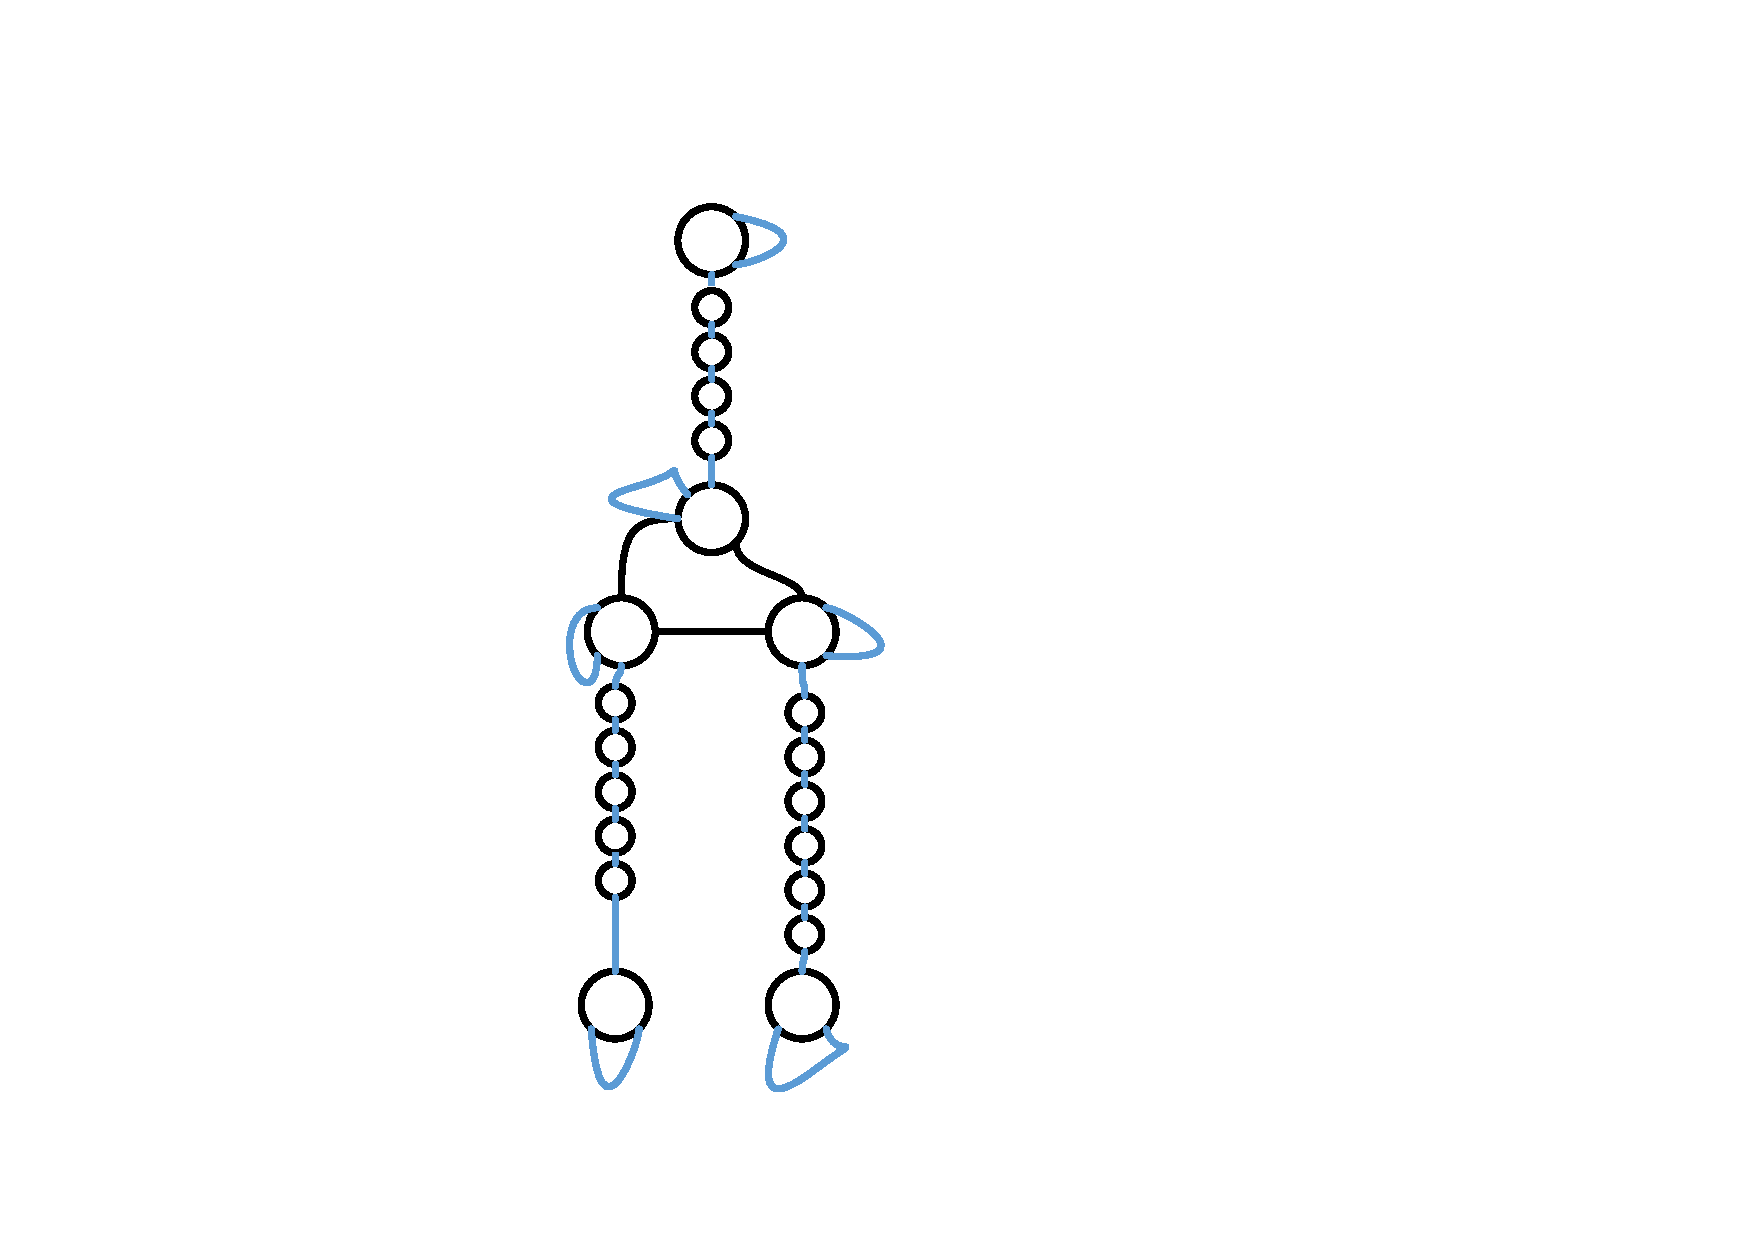
\includegraphics[width=2.5in]{ILP_transfromed_graph}\\
%\caption{transformed Graph G}\label{fig:ILP_transfromed_graph}
%\end{figure}
%
%\begin{figure}
%\centering
%% Requires \usepackage{graphicx}
%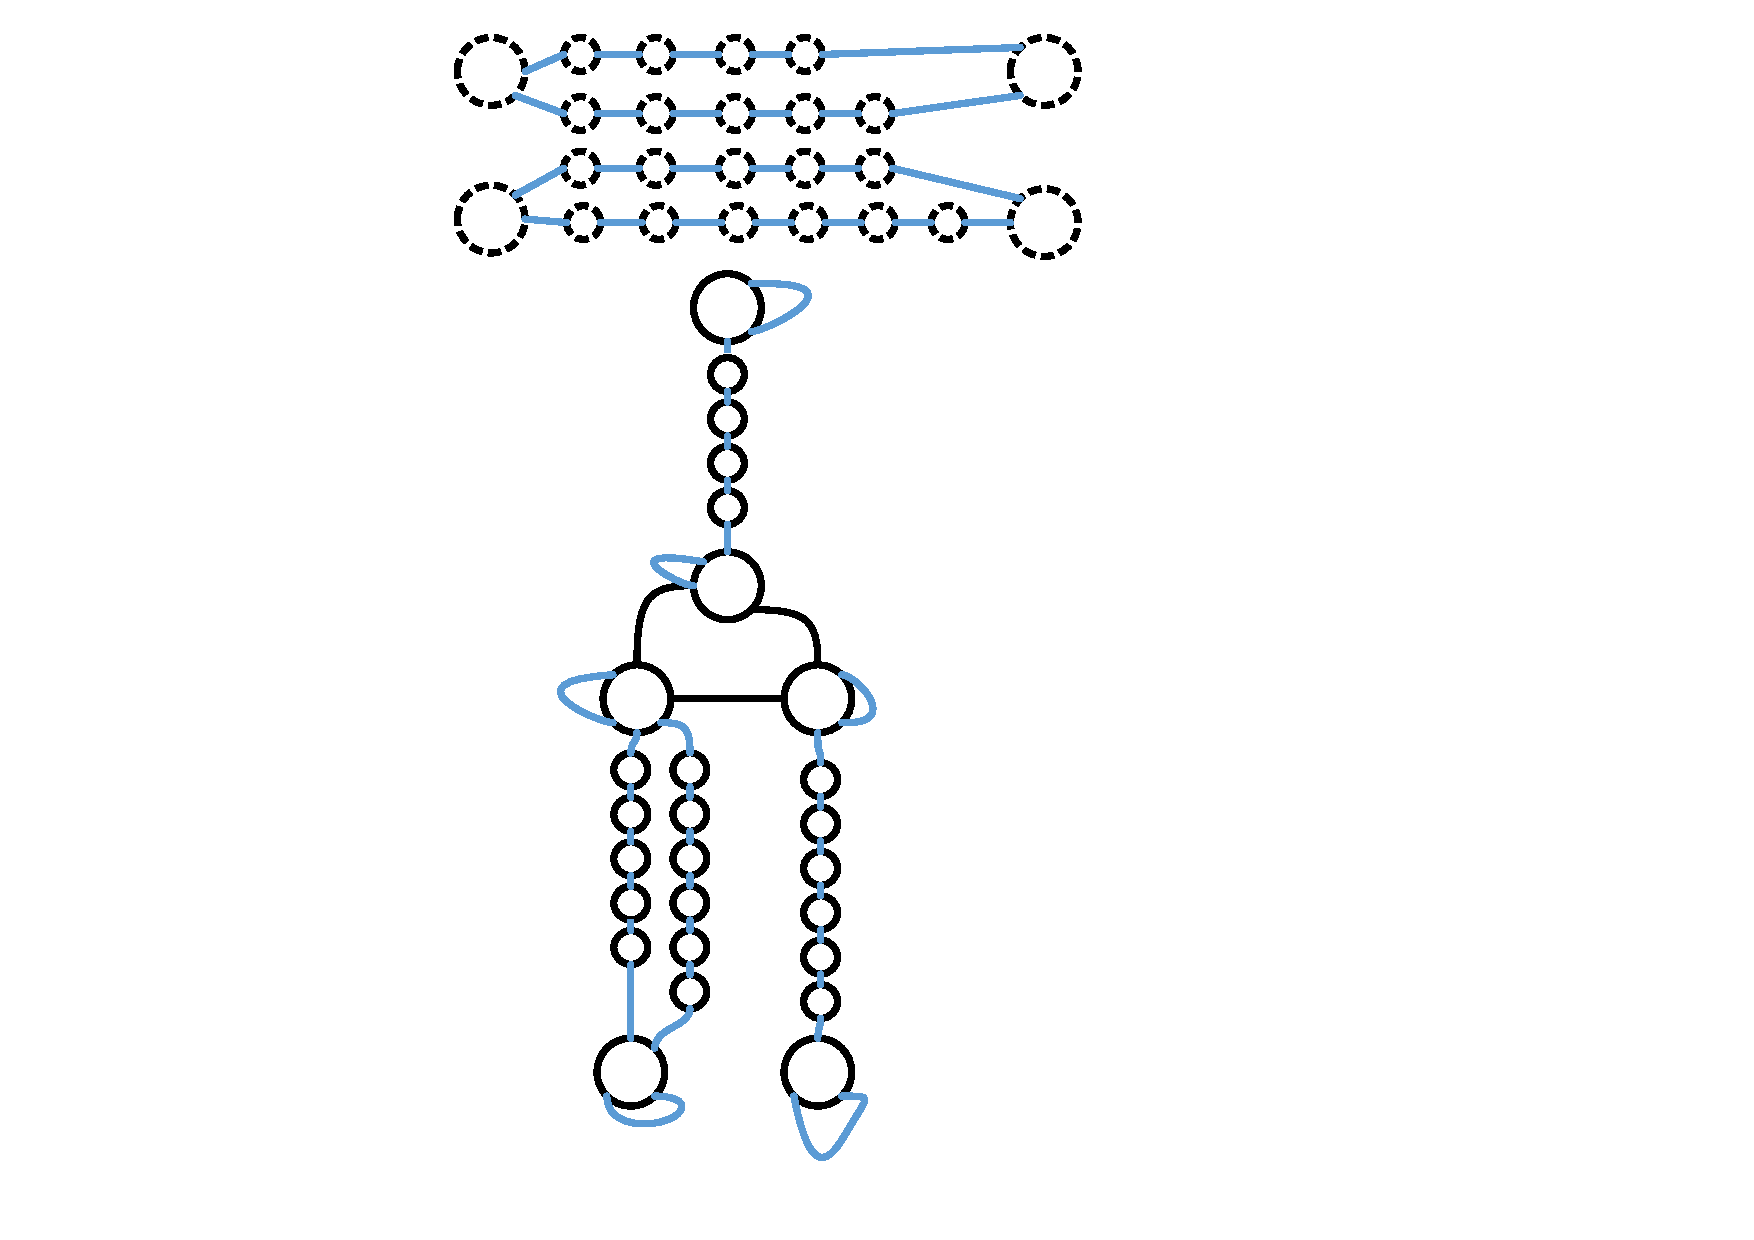
\includegraphics[width=2.5in]{ILP_inserted_augmented_transformed_graph}\\
%\caption{transformed Graph of to be augmented graph G}\label{fig:ILP_inserted_augmented_transformed_graph}
%\end{figure}

\subsection{Objective Function and Approximation}
We seek to minimize the amount of resource used for a SeVN request. The object function of the adapted Integer Programing is then
\begin{align*}
min: C_{new}*\sum_{1\leq i\leq b}A_i+ & M_{migra}*\sum_{1\leq i\leq n}Tran_i  \notag \\
\beta \times(\sum_{1\leq u\leq (n+b)}C^o_{u}- & \sum_{1\leq u\leq n}C_{u}) + \notag \\
\gamma \times(\sum_{1\leq u\leq (n+b),1\leq v\leq (n+b)}B^o_{u,v}- & \sum_{1\leq u\leq n,1\leq v\leq n}B_{u,v})
\end{align*}
where $\beta$, and $\gamma$ are weight about add new node , node's computation and link's bandwith, respectively. To achieve minimize the amount of nodes, respectively, $\beta+\gamma=1$. According to\cite{armbrust2009above,yu2010survivable} the relative cost of computing and bandwidth $\theta=\RelativeCostbetweenComputingBandwidth$, which means $\beta/\gamma=\theta=\RelativeCostbetweenComputingBandwidth$.

The presence of the boolean variables let the integer program of SeVN into a NP-Hard problem. An alterative is to relax the boolean variables to real-value variables between 0 and 1, obtain an approximate virtual node transformation matrix, then rounding decimal value into one or zero and judge the node transformation matrix is logically legal.


Gurobi solver could not able to calculate out the solution because Q matrix of the formulation model is not positive semi-definite (PSD)
